\section{misc.h File Reference}
\label{misc_8h}\index{misc.h@{misc.h}}
{\tt \#include $<$stdio.h$>$}\par
{\tt \#include $<$stdlib.h$>$}\par
{\tt \#include $<$stdarg.h$>$}\par
{\tt \#include $<$string.h$>$}\par
{\tt \#include $<$sys/types.h$>$}\par


Include dependency graph for misc.h:\nopagebreak
\begin{figure}[H]
\begin{center}
\leavevmode
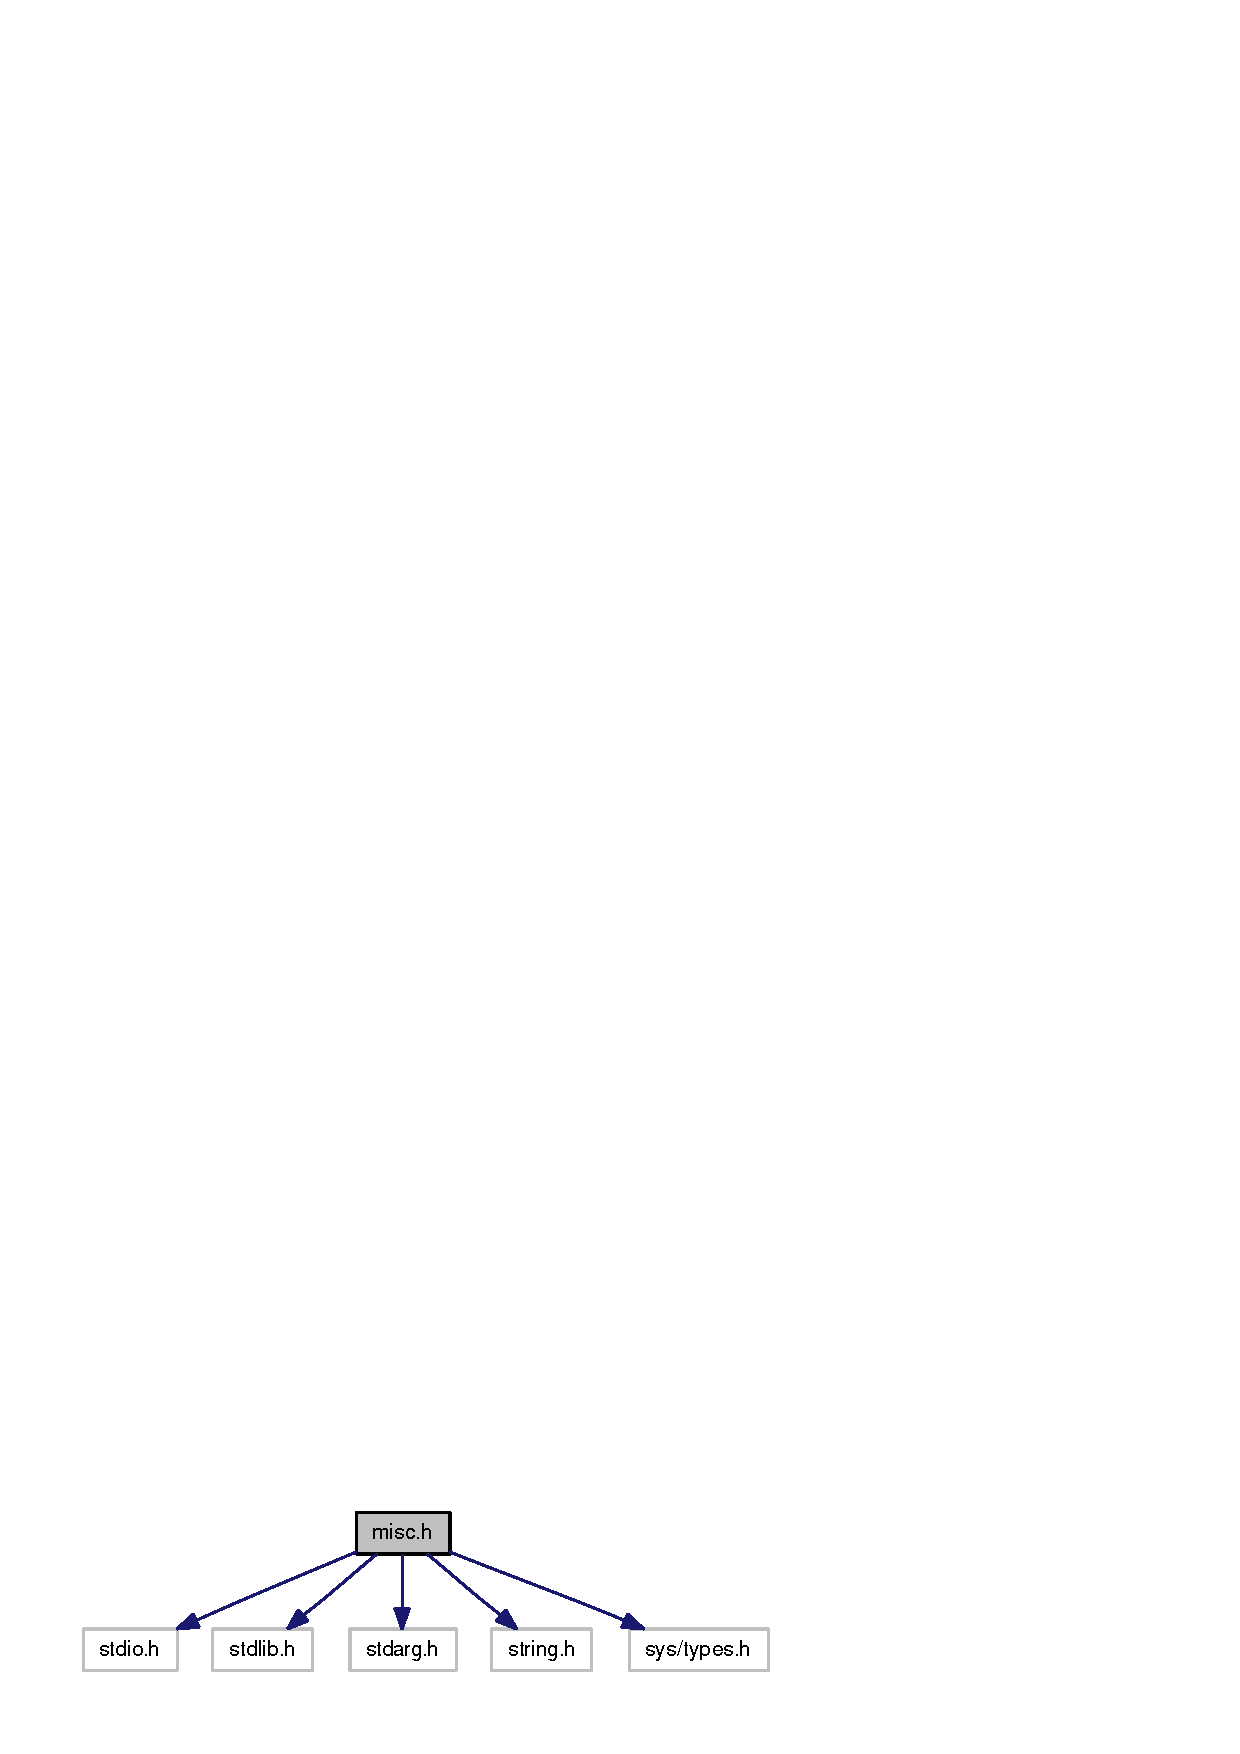
\includegraphics[width=186pt]{misc_8h__incl}
\end{center}
\end{figure}


This graph shows which files directly or indirectly include this file:\nopagebreak
\begin{figure}[H]
\begin{center}
\leavevmode
\includegraphics[width=420pt]{misc_8h__dep__incl}
\end{center}
\end{figure}
\subsection*{Defines}
\begin{CompactItemize}
\item 
\#define {\bf TRUE}~1
\item 
\#define {\bf FALSE}~0
\item 
\#define {\bf MAX}(a, b)~(((a) $<$ (b)) ? (b) : (a))
\item 
\#define {\bf MIN}(a, b)~(((a) $<$ (b)) ? (a) : (b))
\item 
\#define {\bf LLHIGH}(L)~((int)(((L)$>$$>$32) \& 0xffffffff))
\item 
\#define {\bf LLLOW}(L)~((int)((L) \& 0xffffffff))
\item 
\#define {\bf N\_\-ELT}(ARR)~(sizeof(ARR)/sizeof((ARR)[0]))
\item 
\#define {\bf ROUND\_\-UP}(N, ALIGN)~(((N) + ((ALIGN)-1)) \& $\sim$((ALIGN)-1))
\item 
\#define {\bf ROUND\_\-DOWN}(N, ALIGN)~((N) \& $\sim$((ALIGN)-1))
\end{CompactItemize}
\subsection*{Functions}
\begin{CompactItemize}
\item 
void {\bf fatal\_\-hook} (void($\ast$hook\_\-fn)(FILE $\ast$stream))
\item 
void {\bf fatal} (const char $\ast$fmt,...)
\item 
void {\bf panic} (const char $\ast$fmt,...)
\item 
void {\bf warn} (const char $\ast$fmt,...)
\item 
void {\bf info} (const char $\ast$fmt,...)
\item 
static void {\bf debug} (const char $\ast$fmt,...)
\item 
void {\bf mysrand} (const unsigned int seed)
\item 
int {\bf myrand} (void)
\item 
char {\bf mytoupper} (char c)
\item 
char {\bf mytolower} (char c)
\item 
bool {\bf myisalpha} (char c)
\item 
bool {\bf myisdigit} (char c)
\item 
bool {\bf myisspace} (char c)
\item 
bool {\bf myisprint} (char c)
\item 
char $\ast$ {\bf mystrdup} (const char $\ast${\bf s})
\item 
const char $\ast$ {\bf mystrrchr} (const char $\ast${\bf s}, const char c)
\item 
int {\bf mystricmp} (const char $\ast$s1, const char $\ast$s2)
\item 
int {\bf log\_\-base2} (const int n)
\item 
char $\ast$ {\bf elapsed\_\-time} (long sec)
\item 
char $\ast$ {\bf myvsprintf} (char $\ast$obuf, const char $\ast$format, va\_\-list v)
\item 
char $\ast$ {\bf mysprintf} (char $\ast$obuf, const char $\ast$format,...)
\item 
void {\bf myvfprintf} (FILE $\ast$stream, const char $\ast$format, va\_\-list v)
\item 
void {\bf myfprintf} (FILE $\ast$stream, const char $\ast$format,...)
\item 
FILE $\ast$ {\bf gzopen} (const char $\ast$fname, const char $\ast$type)
\item 
void {\bf gzclose} (FILE $\ast$fd)
\item 
int {\bf modinc} (int x, int m)
\item 
int {\bf moddec} (int x, int m)
\item 
int {\bf mod2m} (int x, int m)
\item 
void {\bf memzero} (void $\ast$base, int bytes)
\item 
void {\bf clear\_\-page} (void $\ast$base)
\item 
void {\bf memswap} (void $\ast$p1, void $\ast$p2, size\_\-t num\_\-bytes)
\end{CompactItemize}


\subsection{Define Documentation}
\index{misc.h@{misc.h}!FALSE@{FALSE}}
\index{FALSE@{FALSE}!misc.h@{misc.h}}
\subsubsection[{FALSE}]{\setlength{\rightskip}{0pt plus 5cm}\#define FALSE~0}\label{misc_8h_a93f0eb578d23995850d61f7d61c55c1}




Definition at line 139 of file misc.h.

Referenced by orphan\_\-fn().\index{misc.h@{misc.h}!LLHIGH@{LLHIGH}}
\index{LLHIGH@{LLHIGH}!misc.h@{misc.h}}
\subsubsection[{LLHIGH}]{\setlength{\rightskip}{0pt plus 5cm}\#define LLHIGH(L)~((int)(((L)$>$$>$32) \& 0xffffffff))}\label{misc_8h_3b289ae60231d9e6de0addf1c7780872}




Definition at line 151 of file misc.h.\index{misc.h@{misc.h}!LLLOW@{LLLOW}}
\index{LLLOW@{LLLOW}!misc.h@{misc.h}}
\subsubsection[{LLLOW}]{\setlength{\rightskip}{0pt plus 5cm}\#define LLLOW(L)~((int)((L) \& 0xffffffff))}\label{misc_8h_95321b23a6cc532393c77da65527755f}




Definition at line 152 of file misc.h.\index{misc.h@{misc.h}!MAX@{MAX}}
\index{MAX@{MAX}!misc.h@{misc.h}}
\subsubsection[{MAX}]{\setlength{\rightskip}{0pt plus 5cm}\#define MAX(a, \/  b)~(((a) $<$ (b)) ? (b) : (a))}\label{misc_8h_fa99ec4acc4ecb2dc3c2d05da15d0e3f}




Definition at line 144 of file misc.h.\index{misc.h@{misc.h}!MIN@{MIN}}
\index{MIN@{MIN}!misc.h@{misc.h}}
\subsubsection[{MIN}]{\setlength{\rightskip}{0pt plus 5cm}\#define MIN(a, \/  b)~(((a) $<$ (b)) ? (a) : (b))}\label{misc_8h_3acffbd305ee72dcd4593c0d8af64a4f}




Definition at line 147 of file misc.h.\index{misc.h@{misc.h}!N\_\-ELT@{N\_\-ELT}}
\index{N\_\-ELT@{N\_\-ELT}!misc.h@{misc.h}}
\subsubsection[{N\_\-ELT}]{\setlength{\rightskip}{0pt plus 5cm}\#define N\_\-ELT(ARR)~(sizeof(ARR)/sizeof((ARR)[0]))}\label{misc_8h_0b016faa2169c3e72ef5de317c167530}




Definition at line 155 of file misc.h.\index{misc.h@{misc.h}!ROUND\_\-DOWN@{ROUND\_\-DOWN}}
\index{ROUND\_\-DOWN@{ROUND\_\-DOWN}!misc.h@{misc.h}}
\subsubsection[{ROUND\_\-DOWN}]{\setlength{\rightskip}{0pt plus 5cm}\#define ROUND\_\-DOWN(N, \/  ALIGN)~((N) \& $\sim$((ALIGN)-1))}\label{misc_8h_2e8ad71bbbfff9966240088f9f711927}




Definition at line 159 of file misc.h.\index{misc.h@{misc.h}!ROUND\_\-UP@{ROUND\_\-UP}}
\index{ROUND\_\-UP@{ROUND\_\-UP}!misc.h@{misc.h}}
\subsubsection[{ROUND\_\-UP}]{\setlength{\rightskip}{0pt plus 5cm}\#define ROUND\_\-UP(N, \/  ALIGN)~(((N) + ((ALIGN)-1)) \& $\sim$((ALIGN)-1))}\label{misc_8h_9f347f87831ee6090cb91ac703808537}




Definition at line 158 of file misc.h.\index{misc.h@{misc.h}!TRUE@{TRUE}}
\index{TRUE@{TRUE}!misc.h@{misc.h}}
\subsubsection[{TRUE}]{\setlength{\rightskip}{0pt plus 5cm}\#define TRUE~1}\label{misc_8h_a8cecfc5c5c054d2875c03e77b7be15d}




Definition at line 136 of file misc.h.

Referenced by main(), signal\_\-exit\_\-now(), and signal\_\-sim\_\-stats().

\subsection{Function Documentation}
\index{misc.h@{misc.h}!clear\_\-page@{clear\_\-page}}
\index{clear\_\-page@{clear\_\-page}!misc.h@{misc.h}}
\subsubsection[{clear\_\-page}]{\setlength{\rightskip}{0pt plus 5cm}void clear\_\-page (void $\ast$ {\em base})}\label{misc_8h_d091becb391041832a4ea32756df29b1}


\index{misc.h@{misc.h}!debug@{debug}}
\index{debug@{debug}!misc.h@{misc.h}}
\subsubsection[{debug}]{\setlength{\rightskip}{0pt plus 5cm}static void debug (const char $\ast$ {\em fmt}, \/   {\em ...})\hspace{0.3cm}{\tt  [static]}}\label{misc_8h_61a4c48c5d216baea50bfcef37c3d9fa}




Definition at line 258 of file misc.h.\index{misc.h@{misc.h}!elapsed\_\-time@{elapsed\_\-time}}
\index{elapsed\_\-time@{elapsed\_\-time}!misc.h@{misc.h}}
\subsubsection[{elapsed\_\-time}]{\setlength{\rightskip}{0pt plus 5cm}char$\ast$ elapsed\_\-time (long {\em sec})}\label{misc_8h_4e699a9d021f92b45004b0534715a5d6}


\index{misc.h@{misc.h}!fatal@{fatal}}
\index{fatal@{fatal}!misc.h@{misc.h}}
\subsubsection[{fatal}]{\setlength{\rightskip}{0pt plus 5cm}void fatal (const char $\ast$ {\em fmt}, \/   {\em ...})}\label{misc_8h_677da14e8c4326bde43622f233f1ead3}




Referenced by alloc\_\-create(), bpred\_\-2bC\_\-t::bpred\_\-2bC\_\-t(), bpred\_\-2lev\_\-t::bpred\_\-2lev\_\-t(), bpred\_\-alloyedperceptron\_\-t::bpred\_\-alloyedperceptron\_\-t(), bpred\_\-bimode\_\-t::bpred\_\-bimode\_\-t(), bpred\_\-blg\_\-t::bpred\_\-blg\_\-t(), bpred\_\-btfnt\_\-t::bpred\_\-btfnt\_\-t(), bpred\_\-from\_\-string(), bpred\_\-nottaken\_\-t::bpred\_\-nottaken\_\-t(), bpred\_\-pathneural\_\-t::bpred\_\-pathneural\_\-t(), bpred\_\-perceptron\_\-t::bpred\_\-perceptron\_\-t(), bpred\_\-perfect\_\-t::bpred\_\-perfect\_\-t(), bpred\_\-pwl\_\-t::bpred\_\-pwl\_\-t(), bpred\_\-random\_\-t::bpred\_\-random\_\-t(), bpred\_\-skewed\_\-t::bpred\_\-skewed\_\-t(), bpred\_\-t::bpred\_\-t(), bpred\_\-tage\_\-t::bpred\_\-tage\_\-t(), bpred\_\-taken\_\-t::bpred\_\-taken\_\-t(), bpred\_\-yags\_\-t::bpred\_\-yags\_\-t(), BTB\_\-2levbtac\_\-t::BTB\_\-2levbtac\_\-t(), BTB\_\-btac\_\-t::BTB\_\-btac\_\-t(), BTB\_\-from\_\-string(), BTB\_\-perfect\_\-t::BTB\_\-perfect\_\-t(), bus\_\-create(), cache\_\-create(), cache\_\-create\_\-llc(), cache\_\-get\_\-evictee(), cache\_\-get\_\-evictee\_\-llc(), cache\_\-insert\_\-block(), cache\_\-insert\_\-block\_\-llc(), cache\_\-invalidate(), cache\_\-is\_\-hit(), cache\_\-is\_\-hit\_\-llc(), cache\_\-process(), cache\_\-process\_\-llc(), cache\_\-reg\_\-stats(), core\_\-oracle\_\-t::commit(), commit\_\-create(), core\_\-alloc\_\-DPM\_\-t::core\_\-alloc\_\-DPM\_\-t(), core\_\-alloc\_\-STM\_\-t::core\_\-alloc\_\-STM\_\-t(), core\_\-commit\_\-DPM\_\-t::core\_\-commit\_\-DPM\_\-t(), core\_\-commit\_\-STM\_\-t::core\_\-commit\_\-STM\_\-t(), core\_\-decode\_\-DPM\_\-t::core\_\-decode\_\-DPM\_\-t(), core\_\-decode\_\-STM\_\-t::core\_\-decode\_\-STM\_\-t(), core\_\-exec\_\-DPM\_\-t::core\_\-exec\_\-DPM\_\-t(), core\_\-exec\_\-STM\_\-t::core\_\-exec\_\-STM\_\-t(), core\_\-fetch\_\-DPM\_\-t::core\_\-fetch\_\-DPM\_\-t(), core\_\-fetch\_\-STM\_\-t::core\_\-fetch\_\-STM\_\-t(), core\_\-oracle\_\-t::core\_\-oracle\_\-t(), decode\_\-create(), dram\_\-from\_\-string(), dram\_\-simplescalar\_\-t::dram\_\-simplescalar\_\-t(), dram\_\-simplesdram\_\-t::dram\_\-simplesdram\_\-t(), emergency\_\-recovery(), core\_\-oracle\_\-t::exec(), exec\_\-create(), fetch\_\-create(), fusion\_\-colt\_\-t::fusion\_\-colt\_\-t(), fusion\_\-from\_\-string(), fusion\_\-mcfarling\_\-t::fusion\_\-mcfarling\_\-t(), fusion\_\-multihybrid\_\-t::fusion\_\-multihybrid\_\-t(), fusion\_\-oracle\_\-t::fusion\_\-oracle\_\-t(), fusion\_\-priority\_\-t::fusion\_\-priority\_\-t(), fusion\_\-random\_\-t::fusion\_\-random\_\-t(), fusion\_\-singleton\_\-t::fusion\_\-singleton\_\-t(), BTB\_\-t::get\_\-cache(), fusion\_\-t::get\_\-cache(), bpred\_\-dir\_\-t::get\_\-cache(), core\_\-oracle\_\-t::get\_\-map\_\-node(), core\_\-t::get\_\-odep\_\-link(), core\_\-exec\_\-STM\_\-t::get\_\-readyQ\_\-node(), core\_\-exec\_\-DPM\_\-t::get\_\-readyQ\_\-node(), core\_\-oracle\_\-t::get\_\-spec\_\-mem\_\-node(), bpred\_\-t::get\_\-state\_\-cache(), core\_\-t::get\_\-uop\_\-array(), bpred\_\-t::init\_\-state\_\-cache\_\-pool(), core\_\-fetch\_\-STM\_\-t::jeclear\_\-enqueue(), main(), MC\_\-from\_\-string(), MC\_\-simple\_\-t::MC\_\-simple\_\-t(), memdep\_\-blind\_\-t::memdep\_\-blind\_\-t(), memdep\_\-create(), memdep\_\-lwt\_\-t::memdep\_\-lwt\_\-t(), memdep\_\-none\_\-t::memdep\_\-none\_\-t(), memdep\_\-oracle\_\-t::memdep\_\-oracle\_\-t(), memdep\_\-t::memdep\_\-t(), MSHR\_\-allocate(), prefetch\_\-buffer\_\-create(), prefetch\_\-context\_\-t::prefetch\_\-context\_\-t(), prefetch\_\-create(), prefetch\_\-filter\_\-create(), prefetch\_\-IP\_\-t::prefetch\_\-IP\_\-t(), prefetch\_\-nextline\_\-t::prefetch\_\-nextline\_\-t(), prefetch\_\-stream\_\-t::prefetch\_\-stream\_\-t(), RAS\_\-from\_\-string(), RAS\_\-perfect\_\-t::RAS\_\-perfect\_\-t(), RAS\_\-stack\_\-t::RAS\_\-stack\_\-t(), core\_\-oracle\_\-t::recover(), bpred\_\-t::return\_\-state\_\-cache(), core\_\-commit\_\-STM\_\-t::ROB\_\-fuse\_\-insert(), core\_\-exec\_\-STM\_\-t::RS\_\-fuse\_\-insert(), service\_\-coherence\_\-msg(), uncore\_\-t::setup(), sim\_\-main(), sim\_\-post\_\-init(), core\_\-exec\_\-DPM\_\-t::snatch\_\-back(), core\_\-exec\_\-STM\_\-t::STQ\_\-deallocate\_\-senior(), core\_\-exec\_\-STM\_\-t::STQ\_\-squash\_\-senior(), core\_\-oracle\_\-t::syscall\_\-mem\_\-access(), uncore\_\-t::uncore\_\-t(), core\_\-decode\_\-STM\_\-t::uop\_\-consume(), and core\_\-decode\_\-STM\_\-t::uop\_\-peek().\index{misc.h@{misc.h}!fatal\_\-hook@{fatal\_\-hook}}
\index{fatal\_\-hook@{fatal\_\-hook}!misc.h@{misc.h}}
\subsubsection[{fatal\_\-hook}]{\setlength{\rightskip}{0pt plus 5cm}void fatal\_\-hook (void($\ast$)(FILE $\ast$stream) {\em hook\_\-fn})}\label{misc_8h_cfcad0cdbb8b3f0426d466279f8f821e}




Referenced by main().

Here is the caller graph for this function:\nopagebreak
\begin{figure}[H]
\begin{center}
\leavevmode
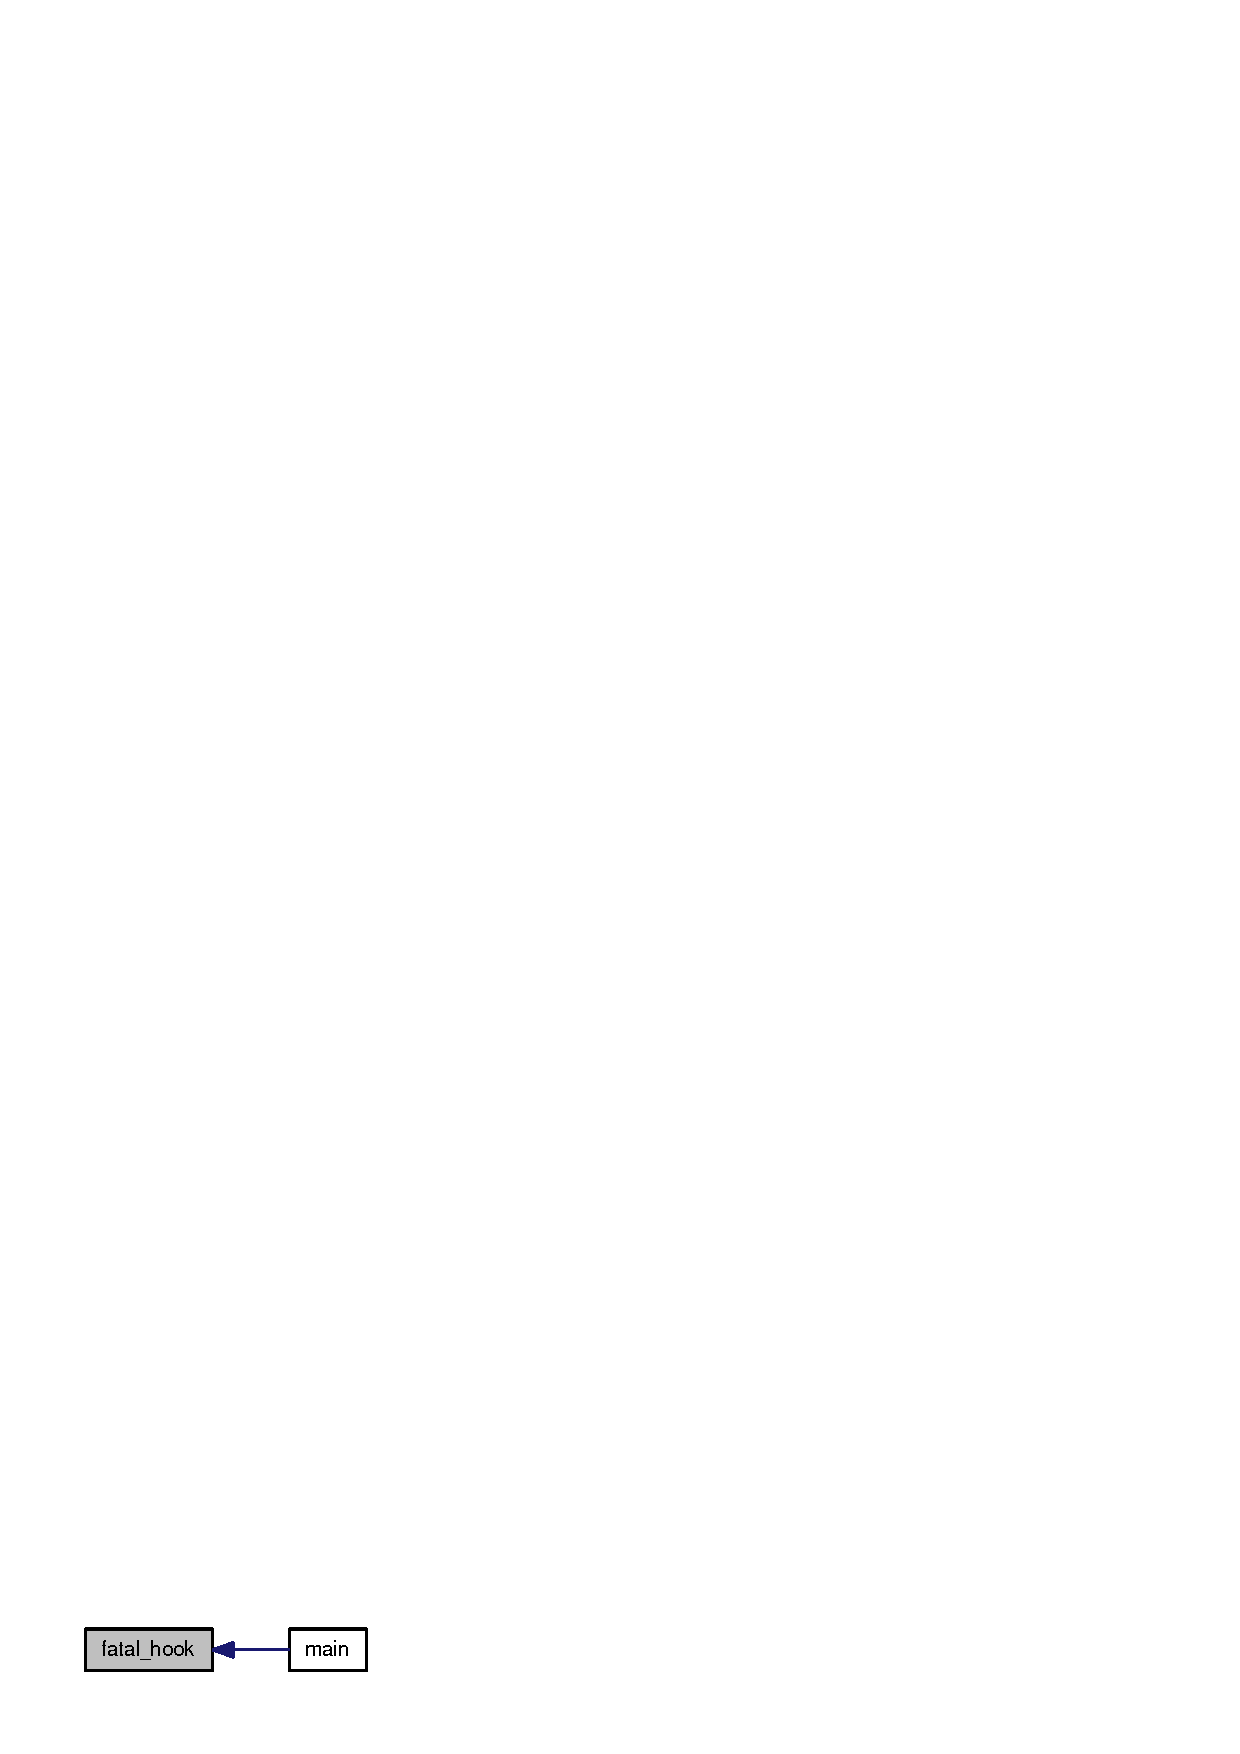
\includegraphics[width=90pt]{misc_8h_cfcad0cdbb8b3f0426d466279f8f821e_icgraph}
\end{center}
\end{figure}
\index{misc.h@{misc.h}!gzclose@{gzclose}}
\index{gzclose@{gzclose}!misc.h@{misc.h}}
\subsubsection[{gzclose}]{\setlength{\rightskip}{0pt plus 5cm}void gzclose (FILE $\ast$ {\em fd})}\label{misc_8h_55b2af0c5efe6baf67e4a2f1439be259}


\index{misc.h@{misc.h}!gzopen@{gzopen}}
\index{gzopen@{gzopen}!misc.h@{misc.h}}
\subsubsection[{gzopen}]{\setlength{\rightskip}{0pt plus 5cm}FILE$\ast$ gzopen (const char $\ast$ {\em fname}, \/  const char $\ast$ {\em type})}\label{misc_8h_96209036d0579b529d206eb0d958662a}


\index{misc.h@{misc.h}!info@{info}}
\index{info@{info}!misc.h@{misc.h}}
\subsubsection[{info}]{\setlength{\rightskip}{0pt plus 5cm}void info (const char $\ast$ {\em fmt}, \/   {\em ...})}\label{misc_8h_38dbef7fdf3b2bd9e8f30dae6f948ce8}


\index{misc.h@{misc.h}!log\_\-base2@{log\_\-base2}}
\index{log\_\-base2@{log\_\-base2}!misc.h@{misc.h}}
\subsubsection[{log\_\-base2}]{\setlength{\rightskip}{0pt plus 5cm}int log\_\-base2 (const int {\em n})}\label{misc_8h_a36cd338e0176d883719b7c69ebc5670}




Referenced by bpred\_\-2lev\_\-t::bpred\_\-2lev\_\-t(), bpred\_\-alloyedperceptron\_\-t::bpred\_\-alloyedperceptron\_\-t(), bpred\_\-bimode\_\-t::bpred\_\-bimode\_\-t(), bpred\_\-blg\_\-t::bpred\_\-blg\_\-t(), bpred\_\-pathneural\_\-t::bpred\_\-pathneural\_\-t(), bpred\_\-perceptron\_\-t::bpred\_\-perceptron\_\-t(), bpred\_\-pwl\_\-t::bpred\_\-pwl\_\-t(), bpred\_\-skewed\_\-t::bpred\_\-skewed\_\-t(), bpred\_\-tage\_\-t::bpred\_\-tage\_\-t(), bpred\_\-yags\_\-t::bpred\_\-yags\_\-t(), BTB\_\-2levbtac\_\-t::BTB\_\-2levbtac\_\-t(), BTB\_\-btac\_\-t::BTB\_\-btac\_\-t(), dram\_\-simplesdram\_\-t::dram\_\-simplesdram\_\-t(), fusion\_\-colt\_\-t::fusion\_\-colt\_\-t(), and prefetch\_\-context\_\-t::prefetch\_\-context\_\-t().

Here is the caller graph for this function:\nopagebreak
\begin{figure}[H]
\begin{center}
\leavevmode
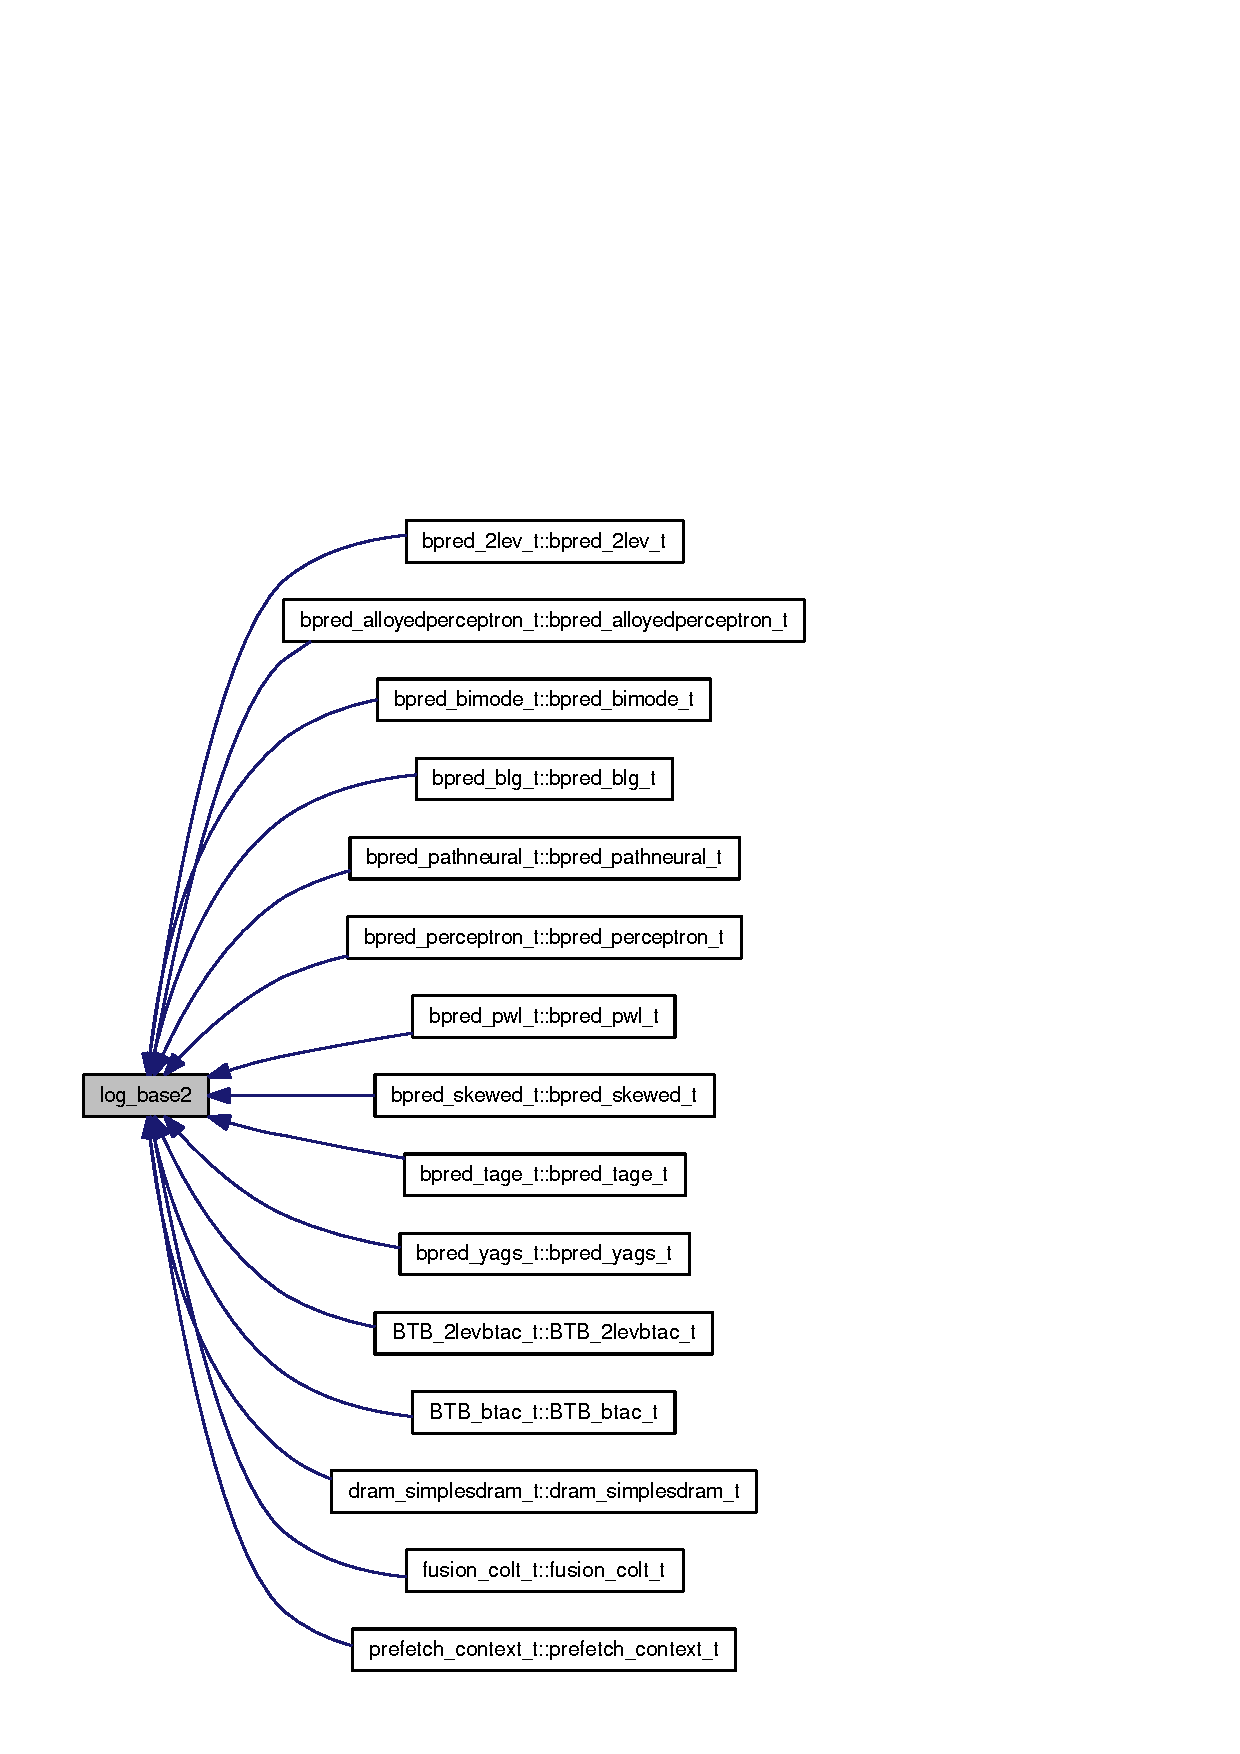
\includegraphics[width=195pt]{misc_8h_a36cd338e0176d883719b7c69ebc5670_icgraph}
\end{center}
\end{figure}
\index{misc.h@{misc.h}!memswap@{memswap}}
\index{memswap@{memswap}!misc.h@{misc.h}}
\subsubsection[{memswap}]{\setlength{\rightskip}{0pt plus 5cm}void memswap (void $\ast$ {\em p1}, \/  void $\ast$ {\em p2}, \/  size\_\-t {\em num\_\-bytes})}\label{misc_8h_e3e882464975b6a22883e91c787d8478}




Referenced by core\_\-exec\_\-STM\_\-t::ALU\_\-heap\_\-balance(), core\_\-exec\_\-STM\_\-t::ALU\_\-heap\_\-remove(), cache\_\-heap\_\-balance(), cache\_\-heap\_\-remove(), fill\_\-heap\_\-balance(), and fill\_\-heap\_\-remove().

Here is the caller graph for this function:\nopagebreak
\begin{figure}[H]
\begin{center}
\leavevmode
\includegraphics[width=420pt]{misc_8h_e3e882464975b6a22883e91c787d8478_icgraph}
\end{center}
\end{figure}
\index{misc.h@{misc.h}!memzero@{memzero}}
\index{memzero@{memzero}!misc.h@{misc.h}}
\subsubsection[{memzero}]{\setlength{\rightskip}{0pt plus 5cm}void memzero (void $\ast$ {\em base}, \/  int {\em bytes})}\label{misc_8h_c0247ae9677929c0d7a34cd197d3e57e}




Referenced by cache\_\-reset\_\-stats(), core\_\-t::core\_\-t(), core\_\-exec\_\-STM\_\-t::LDQ\_\-insert(), core\_\-exec\_\-DPM\_\-t::LDQ\_\-insert(), core\_\-exec\_\-STM\_\-t::LDQ\_\-squash(), core\_\-exec\_\-DPM\_\-t::LDQ\_\-squash(), core\_\-fetch\_\-DPM\_\-t::recover(), core\_\-decode\_\-DPM\_\-t::recover\_\-uopQ(), sim\_\-fastfwd(), sim\_\-pre\_\-init(), core\_\-exec\_\-STM\_\-t::STQ\_\-insert\_\-sta(), core\_\-exec\_\-DPM\_\-t::STQ\_\-insert\_\-sta(), core\_\-exec\_\-DPM\_\-t::STQ\_\-squash\_\-senior(), core\_\-exec\_\-STM\_\-t::STQ\_\-squash\_\-sta(), and core\_\-exec\_\-DPM\_\-t::STQ\_\-squash\_\-sta().

Here is the caller graph for this function:\nopagebreak
\begin{figure}[H]
\begin{center}
\leavevmode
\includegraphics[width=420pt]{misc_8h_c0247ae9677929c0d7a34cd197d3e57e_icgraph}
\end{center}
\end{figure}
\index{misc.h@{misc.h}!mod2m@{mod2m}}
\index{mod2m@{mod2m}!misc.h@{misc.h}}
\subsubsection[{mod2m}]{\setlength{\rightskip}{0pt plus 5cm}int mod2m (int {\em x}, \/  int {\em m})\hspace{0.3cm}{\tt  [inline]}}\label{misc_8h_4c5ce3cf6c3a73be0ec80b5cb93c7159}




Definition at line 355 of file misc.h.

Referenced by zesto\_\-component::downtick\_\-handler(), WBB\_\-insert(), and WBB\_\-victim\_\-insert().

Here is the caller graph for this function:\nopagebreak
\begin{figure}[H]
\begin{center}
\leavevmode
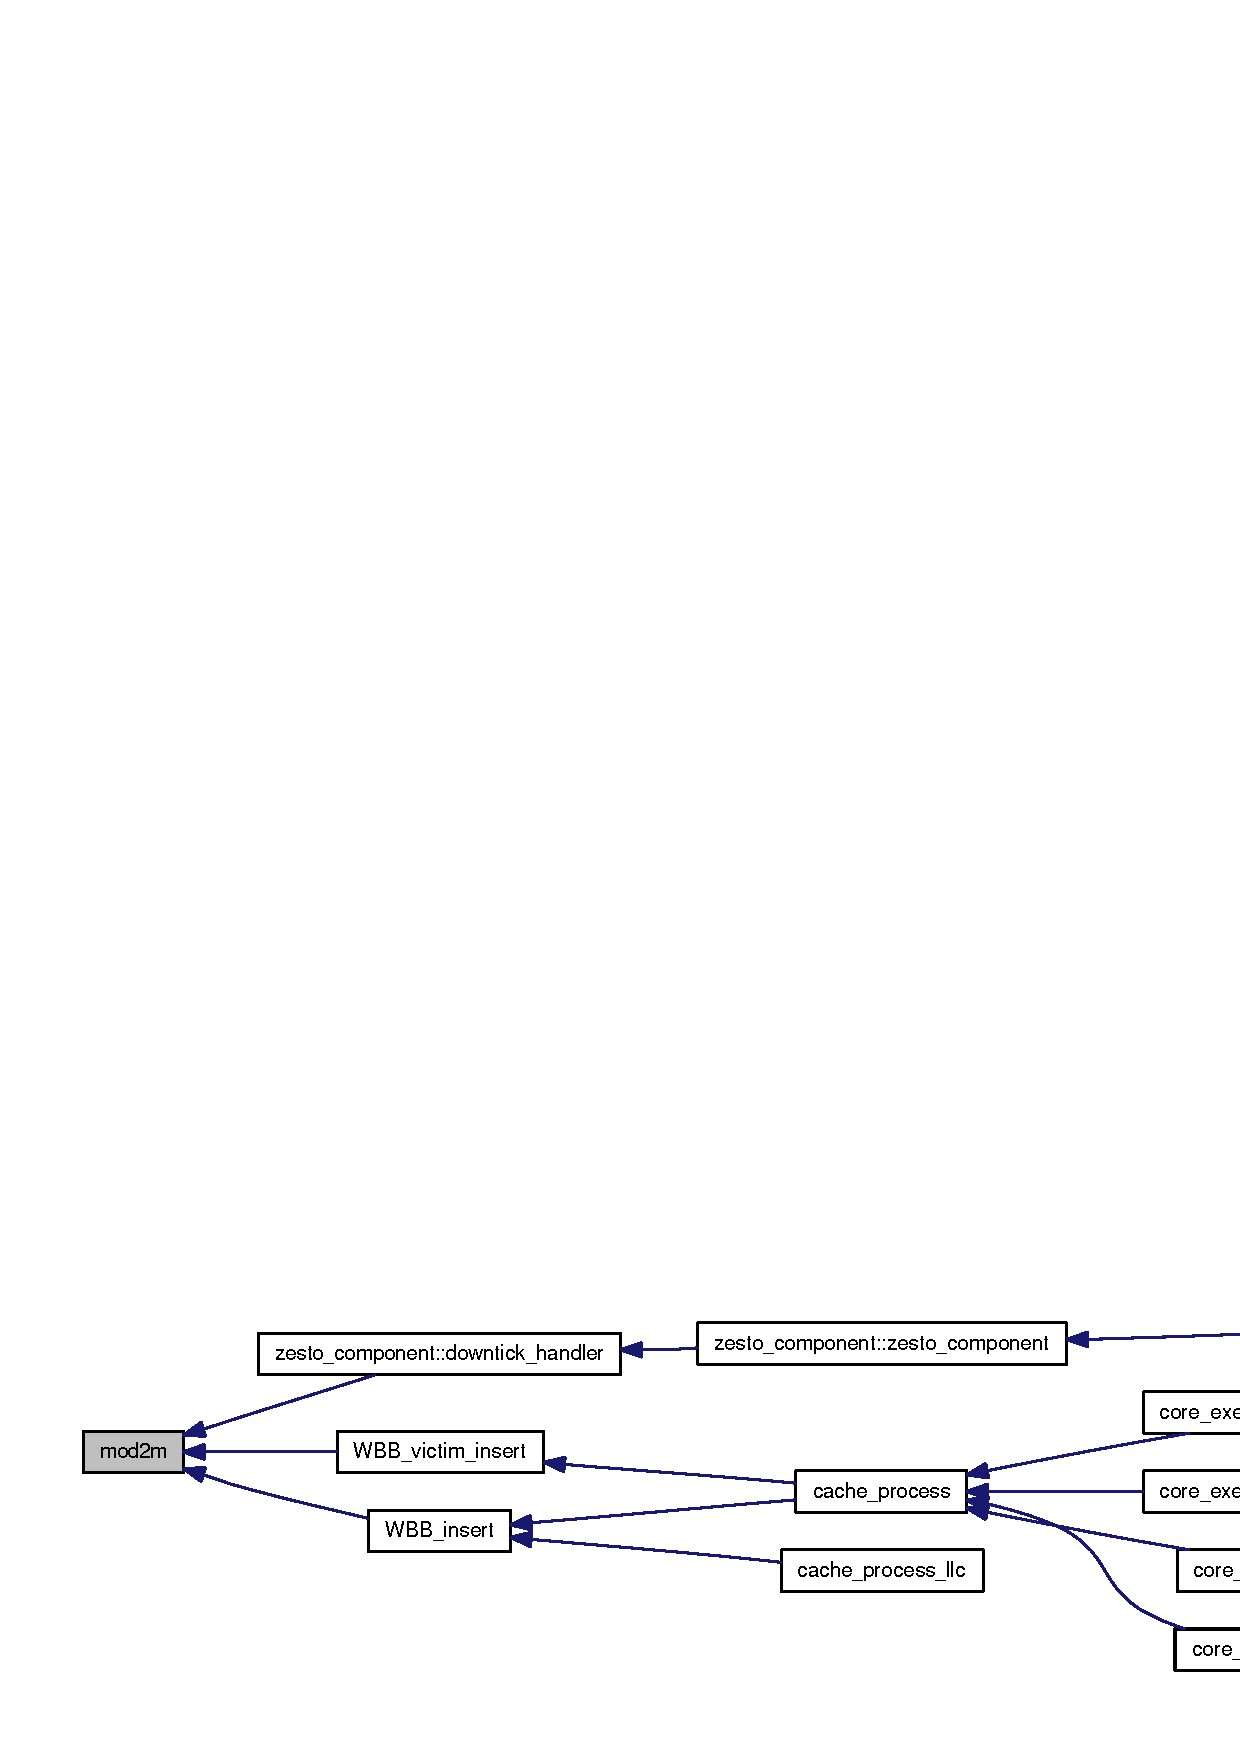
\includegraphics[width=353pt]{misc_8h_4c5ce3cf6c3a73be0ec80b5cb93c7159_icgraph}
\end{center}
\end{figure}
\index{misc.h@{misc.h}!moddec@{moddec}}
\index{moddec@{moddec}!misc.h@{misc.h}}
\subsubsection[{moddec}]{\setlength{\rightskip}{0pt plus 5cm}int moddec (int {\em x}, \/  int {\em m})\hspace{0.3cm}{\tt  [inline]}}\label{misc_8h_e72918bfe3eb9d02e83975f2739a7ab2}




Definition at line 346 of file misc.h.

Referenced by core\_\-fetch\_\-STM\_\-t::byteQ\_\-already\_\-requested(), core\_\-fetch\_\-DPM\_\-t::byteQ\_\-already\_\-requested(), core\_\-exec\_\-STM\_\-t::check\_\-load\_\-issue\_\-conditions(), core\_\-exec\_\-DPM\_\-t::check\_\-load\_\-issue\_\-conditions(), core\_\-oracle\_\-t::complete\_\-flush(), core\_\-exec\_\-STM\_\-t::LDQ\_\-insert(), core\_\-exec\_\-DPM\_\-t::LDQ\_\-insert(), core\_\-exec\_\-STM\_\-t::LDQ\_\-squash(), core\_\-exec\_\-DPM\_\-t::LDQ\_\-squash(), core\_\-exec\_\-STM\_\-t::LDST\_\-exec(), core\_\-exec\_\-DPM\_\-t::LDST\_\-exec(), core\_\-oracle\_\-t::pipe\_\-flush(), core\_\-oracle\_\-t::recover(), core\_\-commit\_\-STM\_\-t::recover(), core\_\-commit\_\-DPM\_\-t::recover(), core\_\-decode\_\-DPM\_\-t::recover\_\-uopQ(), core\_\-fetch\_\-STM\_\-t::step(), core\_\-fetch\_\-DPM\_\-t::step(), core\_\-exec\_\-STM\_\-t::STQ\_\-insert\_\-std(), core\_\-exec\_\-DPM\_\-t::STQ\_\-insert\_\-std(), core\_\-exec\_\-STM\_\-t::STQ\_\-squash\_\-sta(), and core\_\-exec\_\-DPM\_\-t::STQ\_\-squash\_\-sta().

Here is the caller graph for this function:\nopagebreak
\begin{figure}[H]
\begin{center}
\leavevmode
\includegraphics[width=420pt]{misc_8h_e72918bfe3eb9d02e83975f2739a7ab2_icgraph}
\end{center}
\end{figure}
\index{misc.h@{misc.h}!modinc@{modinc}}
\index{modinc@{modinc}!misc.h@{misc.h}}
\subsubsection[{modinc}]{\setlength{\rightskip}{0pt plus 5cm}int modinc (int {\em x}, \/  int {\em m})\hspace{0.3cm}{\tt  [inline]}}\label{misc_8h_ec0decc56f83415e5cd152f876e5dde1}




Definition at line 337 of file misc.h.

Referenced by core\_\-exec\_\-STM\_\-t::ALU\_\-exec(), core\_\-exec\_\-DPM\_\-t::ALU\_\-exec(), core\_\-fetch\_\-STM\_\-t::byteQ\_\-request(), core\_\-fetch\_\-DPM\_\-t::byteQ\_\-request(), cache\_\-get\_\-evictee(), cache\_\-get\_\-evictee\_\-llc(), cache\_\-prefetch(), cache\_\-prefetch\_\-llc(), cache\_\-process(), cache\_\-process\_\-llc(), core\_\-exec\_\-STM\_\-t::check\_\-load\_\-issue\_\-conditions(), core\_\-exec\_\-DPM\_\-t::check\_\-load\_\-issue\_\-conditions(), core\_\-oracle\_\-t::commit(), zesto\_\-component::downtick\_\-handler(), core\_\-oracle\_\-t::exec(), core\_\-exec\_\-STM\_\-t::LDQ\_\-deallocate(), core\_\-exec\_\-DPM\_\-t::LDQ\_\-deallocate(), core\_\-exec\_\-STM\_\-t::LDQ\_\-insert(), core\_\-exec\_\-DPM\_\-t::LDQ\_\-insert(), core\_\-exec\_\-STM\_\-t::LDQ\_\-schedule(), core\_\-exec\_\-DPM\_\-t::LDQ\_\-schedule(), core\_\-fetch\_\-STM\_\-t::Mop\_\-consume(), core\_\-fetch\_\-DPM\_\-t::Mop\_\-consume(), core\_\-oracle\_\-t::next\_\-index(), core\_\-commit\_\-STM\_\-t::ROB\_\-insert(), core\_\-commit\_\-DPM\_\-t::ROB\_\-insert(), core\_\-fetch\_\-STM\_\-t::step(), core\_\-fetch\_\-DPM\_\-t::step(), core\_\-decode\_\-DPM\_\-t::step(), core\_\-commit\_\-STM\_\-t::step(), core\_\-commit\_\-DPM\_\-t::step(), core\_\-exec\_\-DPM\_\-t::STQ\_\-deallocate\_\-senior(), core\_\-exec\_\-STM\_\-t::STQ\_\-deallocate\_\-std(), core\_\-exec\_\-DPM\_\-t::STQ\_\-deallocate\_\-std(), core\_\-exec\_\-STM\_\-t::STQ\_\-insert\_\-sta(), core\_\-exec\_\-DPM\_\-t::STQ\_\-insert\_\-sta(), core\_\-exec\_\-DPM\_\-t::STQ\_\-squash\_\-senior(), core\_\-decode\_\-DPM\_\-t::uop\_\-consume(), and WBB\_\-insert().

Here is the caller graph for this function:\nopagebreak
\begin{figure}[H]
\begin{center}
\leavevmode
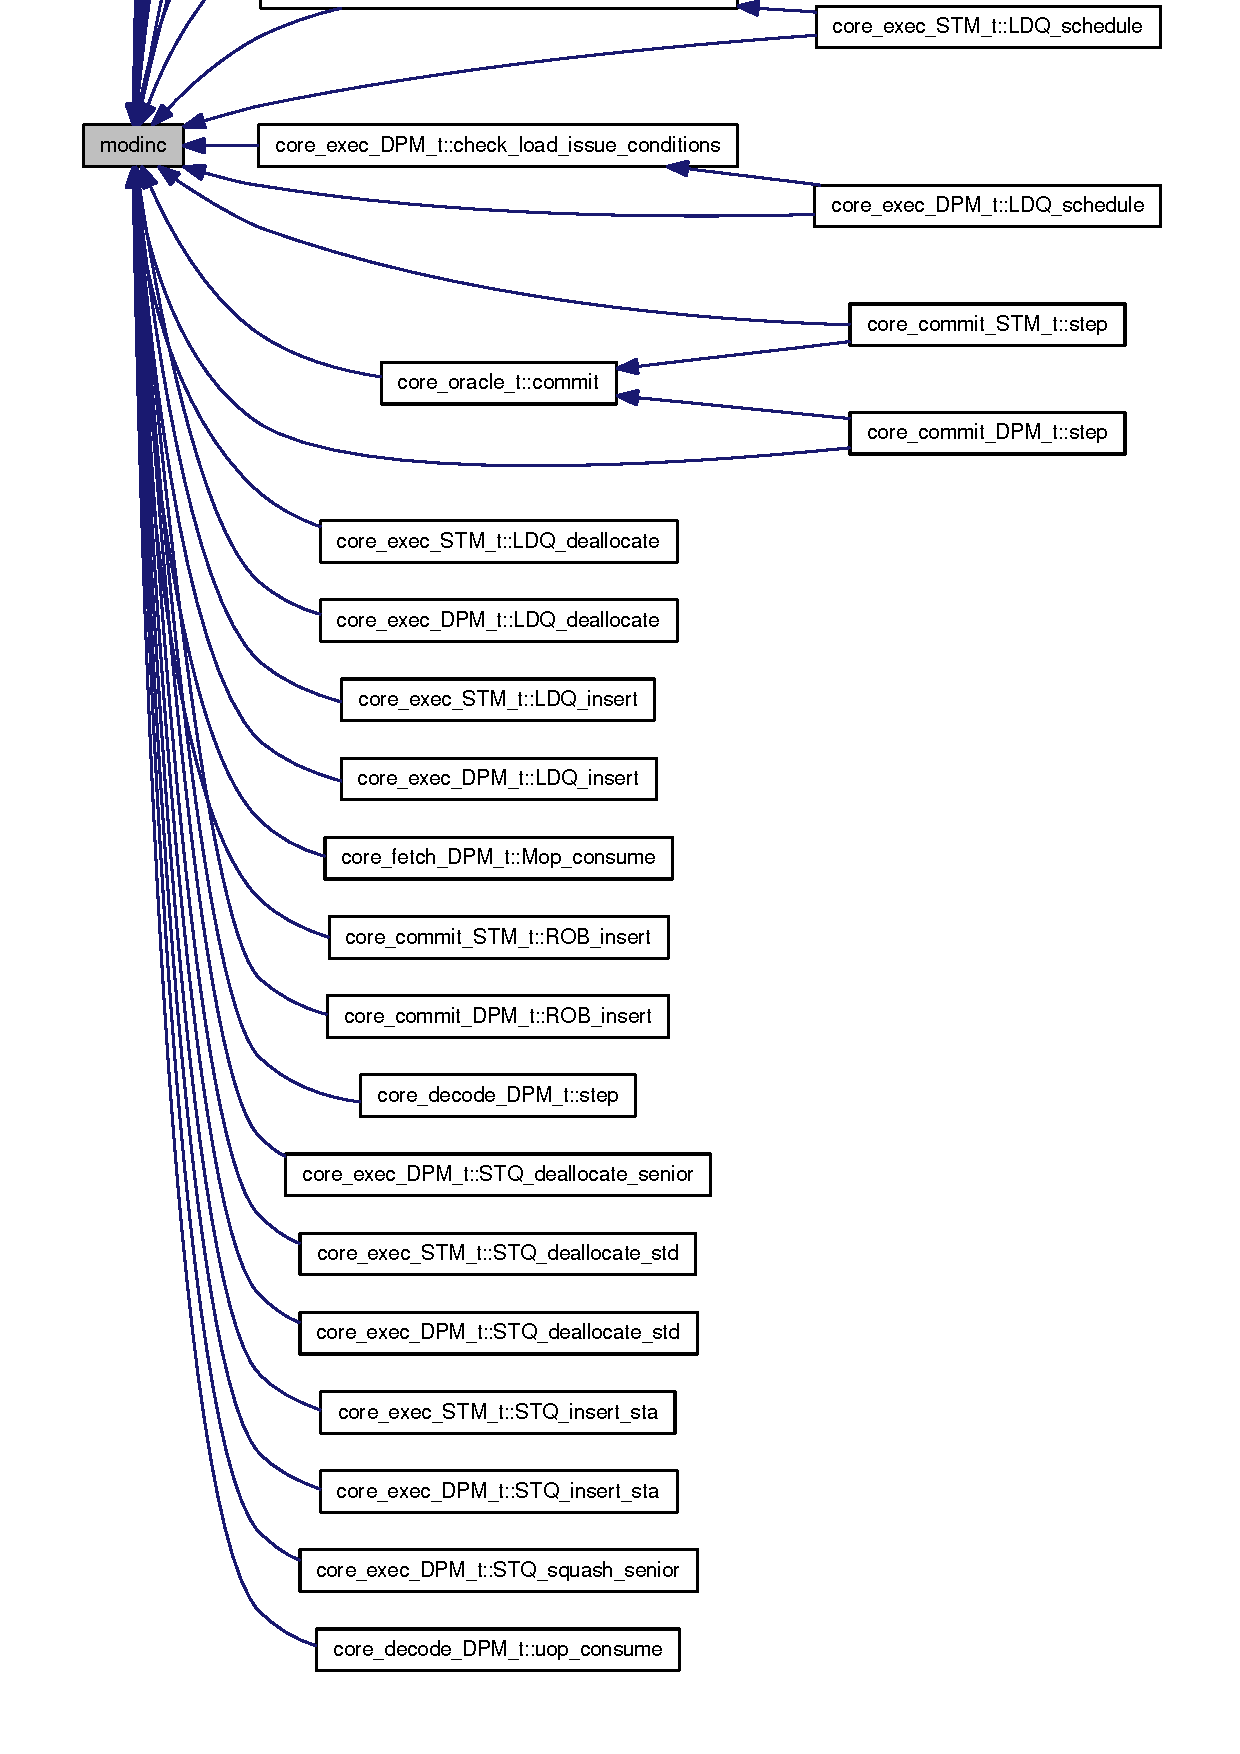
\includegraphics[width=420pt]{misc_8h_ec0decc56f83415e5cd152f876e5dde1_icgraph}
\end{center}
\end{figure}
\index{misc.h@{misc.h}!myfprintf@{myfprintf}}
\index{myfprintf@{myfprintf}!misc.h@{misc.h}}
\subsubsection[{myfprintf}]{\setlength{\rightskip}{0pt plus 5cm}void myfprintf (FILE $\ast$ {\em stream}, \/  const char $\ast$ {\em format}, \/   {\em ...})}\label{misc_8h_43c5d13cbc547afe9061282a5b562e85}


\index{misc.h@{misc.h}!myisalpha@{myisalpha}}
\index{myisalpha@{myisalpha}!misc.h@{misc.h}}
\subsubsection[{myisalpha}]{\setlength{\rightskip}{0pt plus 5cm}bool myisalpha (char {\em c})}\label{misc_8h_8d9098815ece0c95b70d2d208d987d90}


\index{misc.h@{misc.h}!myisdigit@{myisdigit}}
\index{myisdigit@{myisdigit}!misc.h@{misc.h}}
\subsubsection[{myisdigit}]{\setlength{\rightskip}{0pt plus 5cm}bool myisdigit (char {\em c})}\label{misc_8h_94fabc202b35b98525e3d0e9c71af0b6}


\index{misc.h@{misc.h}!myisprint@{myisprint}}
\index{myisprint@{myisprint}!misc.h@{misc.h}}
\subsubsection[{myisprint}]{\setlength{\rightskip}{0pt plus 5cm}bool myisprint (char {\em c})}\label{misc_8h_0587a3c576dceed8a75e6bf3e6b43a74}


\index{misc.h@{misc.h}!myisspace@{myisspace}}
\index{myisspace@{myisspace}!misc.h@{misc.h}}
\subsubsection[{myisspace}]{\setlength{\rightskip}{0pt plus 5cm}bool myisspace (char {\em c})}\label{misc_8h_3ee813d5c2fd0067bf0aa95c4be26add}


\index{misc.h@{misc.h}!myrand@{myrand}}
\index{myrand@{myrand}!misc.h@{misc.h}}
\subsubsection[{myrand}]{\setlength{\rightskip}{0pt plus 5cm}int myrand (void)}\label{misc_8h_371debed7f5b7d78252c57128b8d5e88}


\index{misc.h@{misc.h}!mysprintf@{mysprintf}}
\index{mysprintf@{mysprintf}!misc.h@{misc.h}}
\subsubsection[{mysprintf}]{\setlength{\rightskip}{0pt plus 5cm}char$\ast$ mysprintf (char $\ast$ {\em obuf}, \/  const char $\ast$ {\em format}, \/   {\em ...})}\label{misc_8h_0b20cf34e1f8fd6145a84939ebf83117}


\index{misc.h@{misc.h}!mysrand@{mysrand}}
\index{mysrand@{mysrand}!misc.h@{misc.h}}
\subsubsection[{mysrand}]{\setlength{\rightskip}{0pt plus 5cm}void mysrand (const unsigned int {\em seed})}\label{misc_8h_f7918804a6274603680ea16fd10fdc62}




Referenced by main().

Here is the caller graph for this function:\nopagebreak
\begin{figure}[H]
\begin{center}
\leavevmode
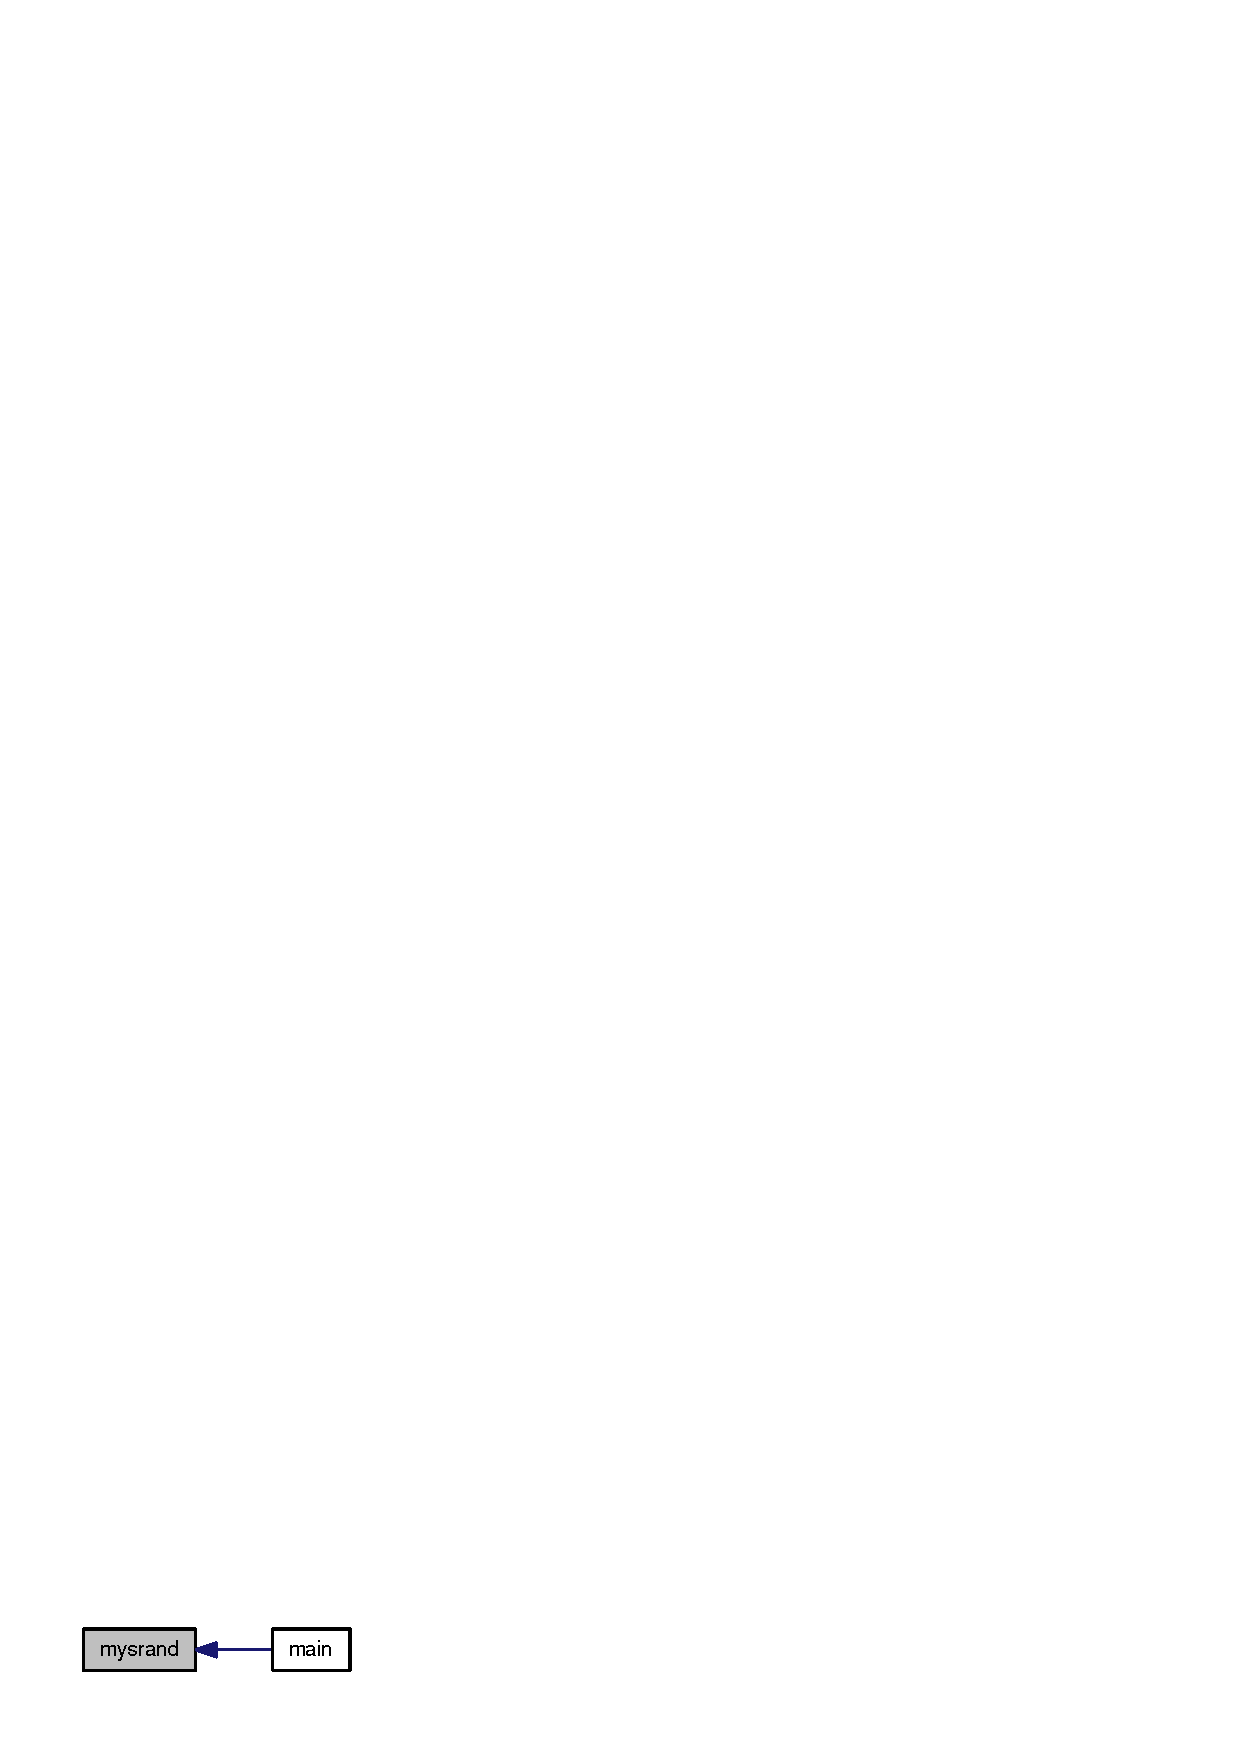
\includegraphics[width=86pt]{misc_8h_f7918804a6274603680ea16fd10fdc62_icgraph}
\end{center}
\end{figure}
\index{misc.h@{misc.h}!mystrdup@{mystrdup}}
\index{mystrdup@{mystrdup}!misc.h@{misc.h}}
\subsubsection[{mystrdup}]{\setlength{\rightskip}{0pt plus 5cm}char$\ast$ mystrdup (const char $\ast$ {\em s})}\label{misc_8h_aec695d4d3f73b13b968950d7857116d}


\index{misc.h@{misc.h}!mystricmp@{mystricmp}}
\index{mystricmp@{mystricmp}!misc.h@{misc.h}}
\subsubsection[{mystricmp}]{\setlength{\rightskip}{0pt plus 5cm}int mystricmp (const char $\ast$ {\em s1}, \/  const char $\ast$ {\em s2})}\label{misc_8h_2b5de5706c409f5bb169eafa7ced66d8}


\index{misc.h@{misc.h}!mystrrchr@{mystrrchr}}
\index{mystrrchr@{mystrrchr}!misc.h@{misc.h}}
\subsubsection[{mystrrchr}]{\setlength{\rightskip}{0pt plus 5cm}const char$\ast$ mystrrchr (const char $\ast$ {\em s}, \/  const char {\em c})}\label{misc_8h_422c7e3eab812cae01eaa8d33d5c58d3}


\index{misc.h@{misc.h}!mytolower@{mytolower}}
\index{mytolower@{mytolower}!misc.h@{misc.h}}
\subsubsection[{mytolower}]{\setlength{\rightskip}{0pt plus 5cm}char mytolower (char {\em c})}\label{misc_8h_a400d7148b23b4458a7dd87fc590d780}




Referenced by BTB\_\-2levbtac\_\-t::BTB\_\-2levbtac\_\-t(), and BTB\_\-btac\_\-t::BTB\_\-btac\_\-t().

Here is the caller graph for this function:\nopagebreak
\begin{figure}[H]
\begin{center}
\leavevmode
\includegraphics[width=151pt]{misc_8h_a400d7148b23b4458a7dd87fc590d780_icgraph}
\end{center}
\end{figure}
\index{misc.h@{misc.h}!mytoupper@{mytoupper}}
\index{mytoupper@{mytoupper}!misc.h@{misc.h}}
\subsubsection[{mytoupper}]{\setlength{\rightskip}{0pt plus 5cm}char mytoupper (char {\em c})}\label{misc_8h_e9332e6ace7e2352b856c2a76bd9ef43}




Referenced by cache\_\-create(), cache\_\-create\_\-llc(), core\_\-exec\_\-DPM\_\-t::core\_\-exec\_\-DPM\_\-t(), core\_\-exec\_\-STM\_\-t::core\_\-exec\_\-STM\_\-t(), and uncore\_\-t::uncore\_\-t().

Here is the caller graph for this function:\nopagebreak
\begin{figure}[H]
\begin{center}
\leavevmode
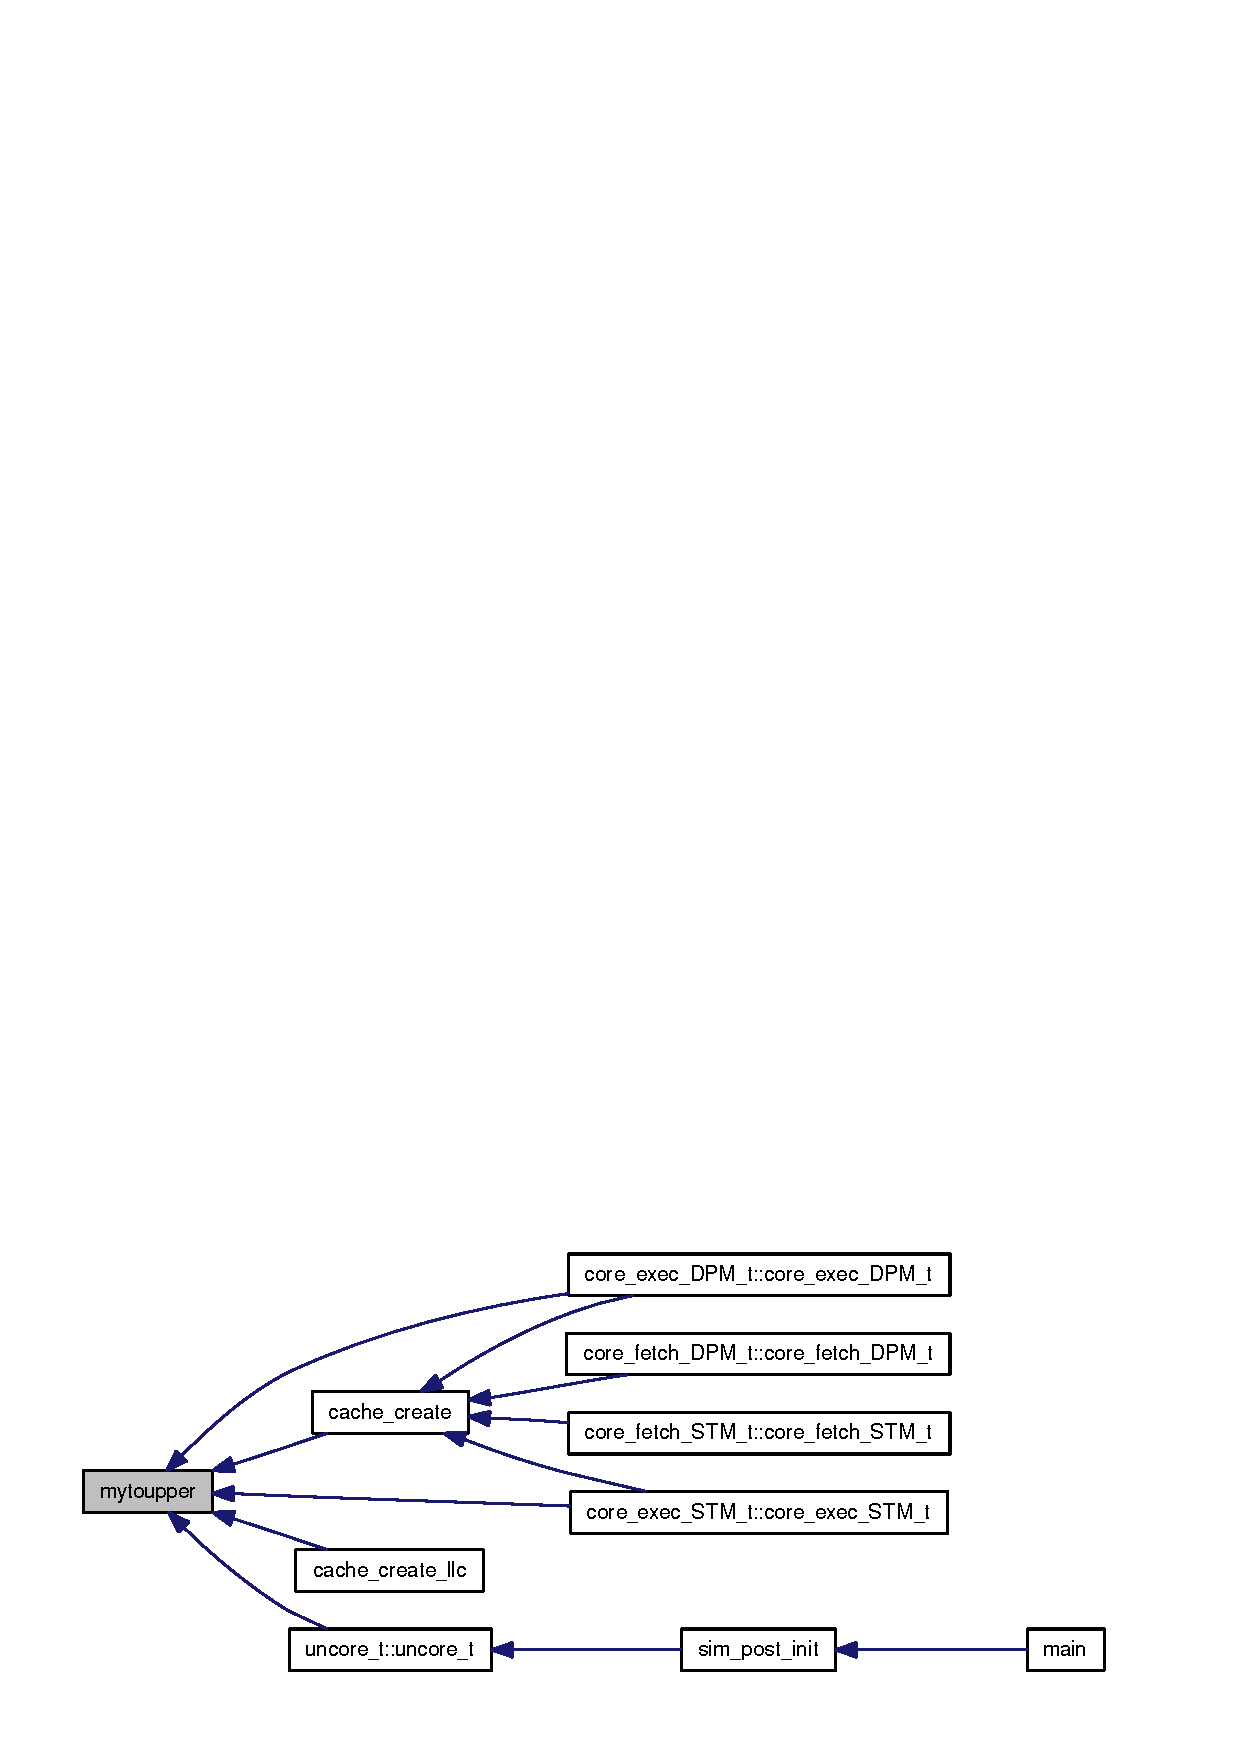
\includegraphics[width=267pt]{misc_8h_e9332e6ace7e2352b856c2a76bd9ef43_icgraph}
\end{center}
\end{figure}
\index{misc.h@{misc.h}!myvfprintf@{myvfprintf}}
\index{myvfprintf@{myvfprintf}!misc.h@{misc.h}}
\subsubsection[{myvfprintf}]{\setlength{\rightskip}{0pt plus 5cm}void myvfprintf (FILE $\ast$ {\em stream}, \/  const char $\ast$ {\em format}, \/  va\_\-list {\em v})}\label{misc_8h_aa0d7ecda2812ae947ffbd08324e54ad}


\index{misc.h@{misc.h}!myvsprintf@{myvsprintf}}
\index{myvsprintf@{myvsprintf}!misc.h@{misc.h}}
\subsubsection[{myvsprintf}]{\setlength{\rightskip}{0pt plus 5cm}char$\ast$ myvsprintf (char $\ast$ {\em obuf}, \/  const char $\ast$ {\em format}, \/  va\_\-list {\em v})}\label{misc_8h_e90a30a33cca2218c0f0435e7f43f629}


\index{misc.h@{misc.h}!panic@{panic}}
\index{panic@{panic}!misc.h@{misc.h}}
\subsubsection[{panic}]{\setlength{\rightskip}{0pt plus 5cm}void panic (const char $\ast$ {\em fmt}, \/   {\em ...})}\label{misc_8h_d1f1a1dc0581a11b597453f148106393}




Referenced by core\_\-oracle\_\-t::exec().

Here is the caller graph for this function:\nopagebreak
\begin{figure}[H]
\begin{center}
\leavevmode
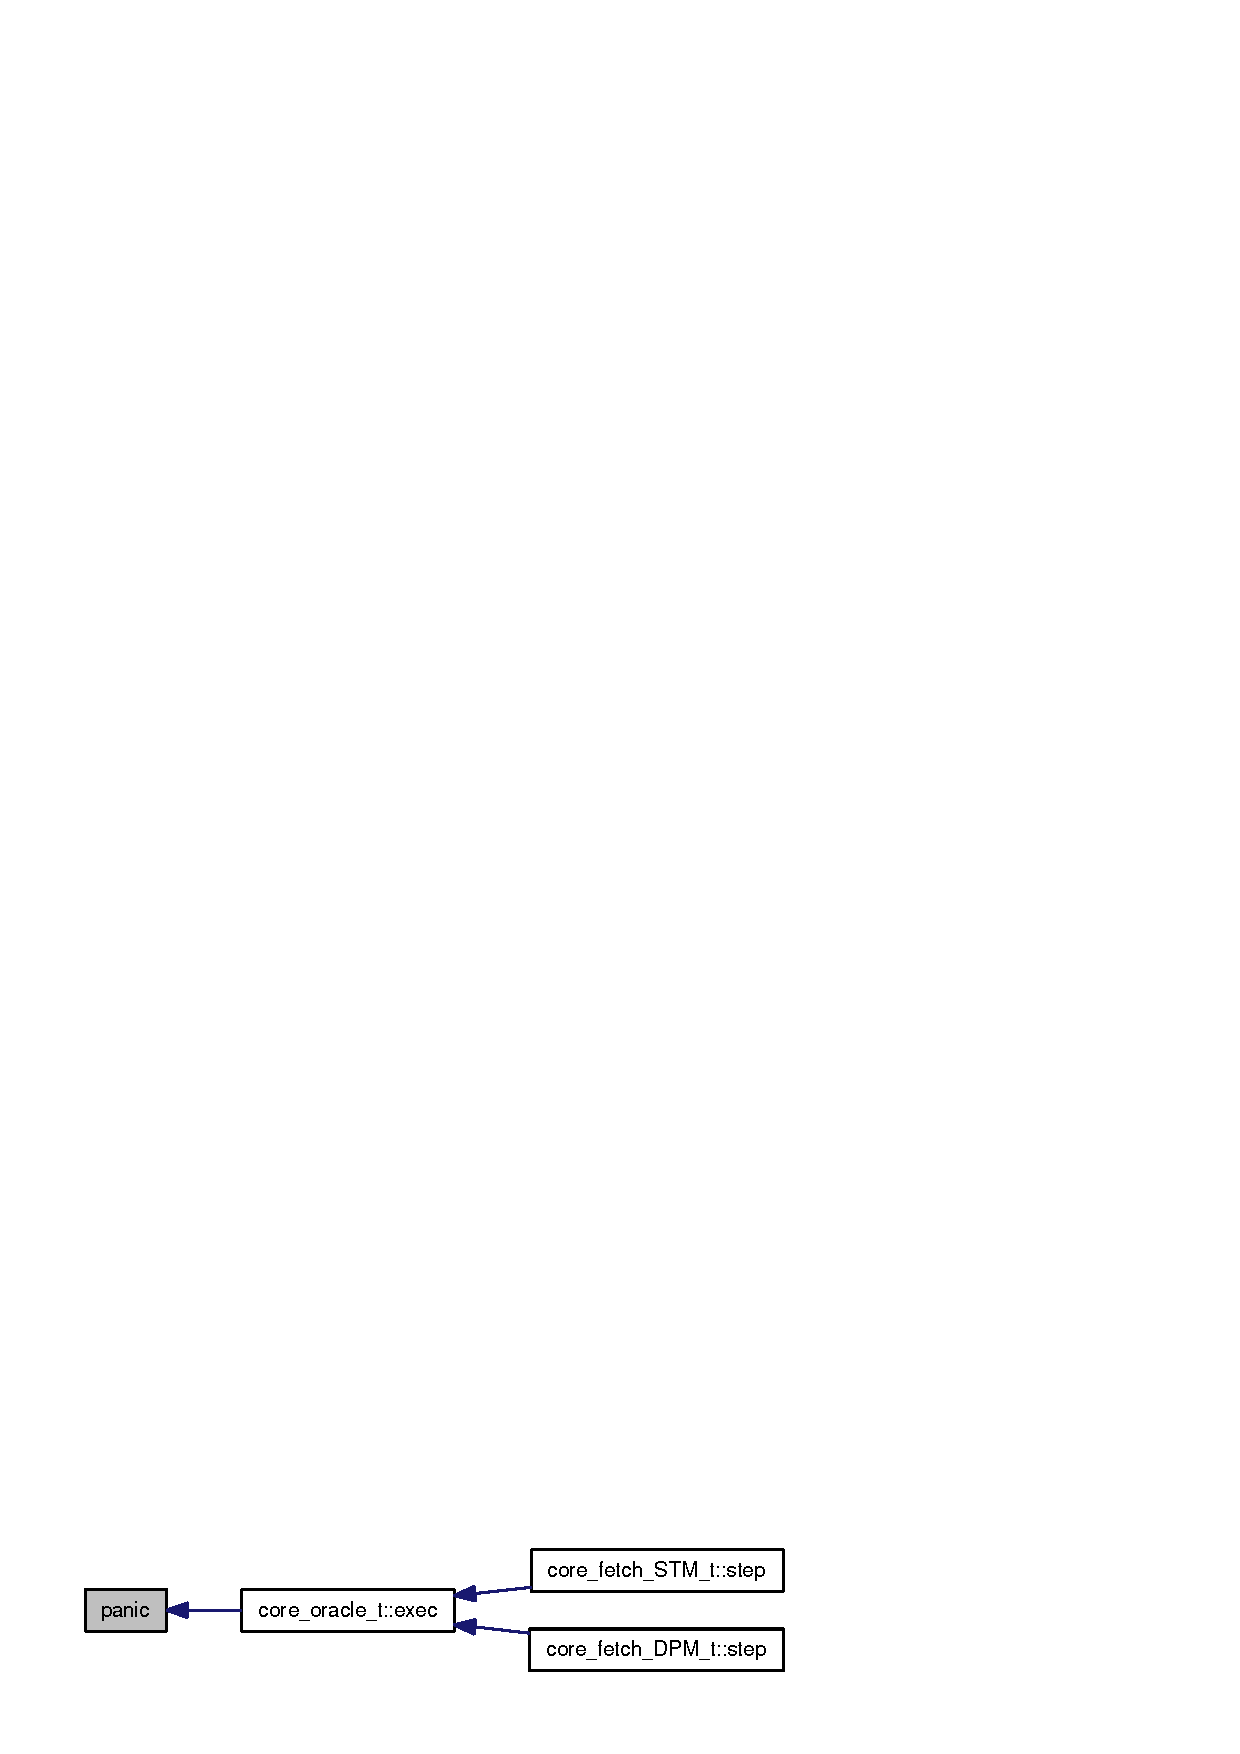
\includegraphics[width=190pt]{misc_8h_d1f1a1dc0581a11b597453f148106393_icgraph}
\end{center}
\end{figure}
\index{misc.h@{misc.h}!warn@{warn}}
\index{warn@{warn}!misc.h@{misc.h}}
\subsubsection[{warn}]{\setlength{\rightskip}{0pt plus 5cm}void warn (const char $\ast$ {\em fmt}, \/   {\em ...})}\label{misc_8h_f80d19f1297a11626fab61a248959c71}




Referenced by core\_\-oracle\_\-t::exec(), core\_\-exec\_\-STM\_\-t::LDST\_\-exec(), core\_\-exec\_\-DPM\_\-t::LDST\_\-exec(), core\_\-exec\_\-STM\_\-t::load\_\-writeback(), core\_\-exec\_\-DPM\_\-t::load\_\-writeback(), core\_\-commit\_\-STM\_\-t::step(), and core\_\-commit\_\-DPM\_\-t::step().

Here is the caller graph for this function:\nopagebreak
\begin{figure}[H]
\begin{center}
\leavevmode
\includegraphics[width=353pt]{misc_8h_f80d19f1297a11626fab61a248959c71_icgraph}
\end{center}
\end{figure}
